\documentclass{standalone}
\usepackage{tikz}
\usetikzlibrary{patterns, positioning}

\begin{document}
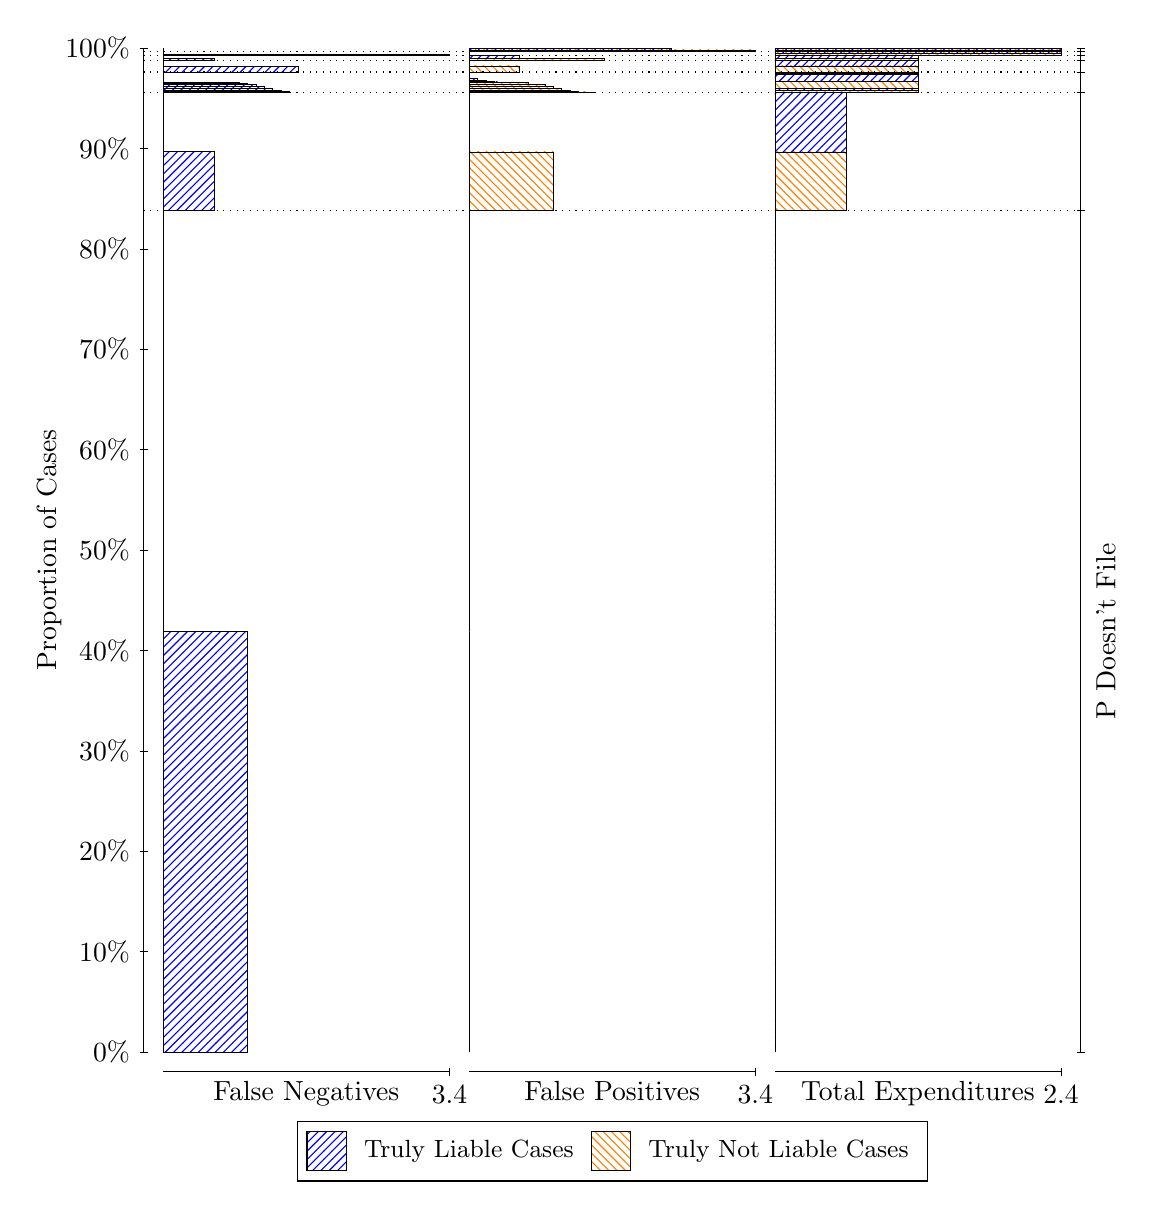
\begin{tikzpicture}
\draw[black, very thin] (1.5,1.75) -- (1.5,14.5);
\node[rotate=90, anchor=center] at (0.3, 8.125) {Proportion of Cases};
\draw[black, very thin] (1.45,1.75) -- (1.55,1.75);
\node[anchor=east] at (1.45, 1.75) {0\%};
\draw[black, very thin] (1.45,3.025) -- (1.55,3.025);
\node[anchor=east] at (1.45, 3.025) {10\%};
\draw[black, very thin] (1.45,4.3) -- (1.55,4.3);
\node[anchor=east] at (1.45, 4.3) {20\%};
\draw[black, very thin] (1.45,5.575) -- (1.55,5.575);
\node[anchor=east] at (1.45, 5.575) {30\%};
\draw[black, very thin] (1.45,6.85) -- (1.55,6.85);
\node[anchor=east] at (1.45, 6.85) {40\%};
\draw[black, very thin] (1.45,8.125) -- (1.55,8.125);
\node[anchor=east] at (1.45, 8.125) {50\%};
\draw[black, very thin] (1.45,9.4) -- (1.55,9.4);
\node[anchor=east] at (1.45, 9.4) {60\%};
\draw[black, very thin] (1.45,10.675) -- (1.55,10.675);
\node[anchor=east] at (1.45, 10.675) {70\%};
\draw[black, very thin] (1.45,11.95) -- (1.55,11.95);
\node[anchor=east] at (1.45, 11.95) {80\%};
\draw[black, very thin] (1.45,13.225) -- (1.55,13.225);
\node[anchor=east] at (1.45, 13.225) {90\%};
\draw[black, very thin] (1.45,14.5) -- (1.55,14.5);
\node[anchor=east] at (1.45, 14.5) {100\%};

\draw[black, very thin] (13.4,1.75) -- (13.4,14.5);
\draw[black, very thin] (13.35,1.75) -- (13.45,1.75);
\node[anchor=west] at (13.35, 1.75) {};
\draw[black, very thin] (13.35,12.435) -- (13.45,12.435);
\node[anchor=west] at (13.35, 12.435) {};
\draw[black, very thin] (13.35,13.935) -- (13.45,13.935);
\node[anchor=west] at (13.35, 13.935) {};
\draw[black, very thin] (13.35,14.195) -- (13.45,14.195);
\node[anchor=west] at (13.35, 14.195) {};
\draw[black, very thin] (13.35,14.339) -- (13.45,14.339);
\node[anchor=west] at (13.35, 14.339) {};
\draw[black, very thin] (13.35,14.402) -- (13.45,14.402);
\node[anchor=west] at (13.35, 14.402) {};
\draw[black, very thin] (13.35,14.46) -- (13.45,14.46);
\node[anchor=west] at (13.35, 14.46) {};
\draw[black, very thin] (13.35,14.5) -- (13.45,14.5);
\node[anchor=west] at (13.35, 14.5) {};

\draw[black, very thin, pattern color=blue, pattern=north east lines] (1.75,1.75) rectangle (2.8186,7.0924);
\draw[black, very thin, pattern color=orange, pattern=north west lines] (1.75,7.0924) rectangle (1.75,12.435);
\draw[black, very thin, pattern color=blue, pattern=north east lines] (1.75,12.435) rectangle (2.3912,13.189);
\draw[black, very thin, pattern color=orange, pattern=north west lines] (1.75,13.189) rectangle (1.75,13.935);
\draw[black, very thin, pattern color=blue, pattern=north east lines] (1.75,13.935) rectangle (3.3529,13.953);
\draw[black, very thin, pattern color=blue, pattern=north east lines] (1.75,13.953) rectangle (3.2461,13.96);
\draw[black, very thin, pattern color=blue, pattern=north east lines] (1.75,13.96) rectangle (3.1392,13.988);
\draw[black, very thin, pattern color=blue, pattern=north east lines] (1.75,13.988) rectangle (3.0324,14.014);
\draw[black, very thin, pattern color=blue, pattern=north east lines] (1.75,14.014) rectangle (2.9255,14.042);
\draw[black, very thin, pattern color=blue, pattern=north east lines] (1.75,14.042) rectangle (2.8186,14.052);
\draw[black, very thin, pattern color=blue, pattern=north east lines] (1.75,14.052) rectangle (2.7118,14.06);
\draw[black, very thin, pattern color=blue, pattern=north east lines] (1.75,14.06) rectangle (2.6049,14.063);
\draw[black, very thin, pattern color=blue, pattern=north east lines] (1.75,14.063) rectangle (2.498,14.067);
\draw[black, very thin, pattern color=orange, pattern=north west lines] (1.75,14.067) rectangle (1.75,14.195);
\draw[black, very thin, pattern color=blue, pattern=north east lines] (1.75,14.195) rectangle (3.4598,14.263);
\draw[black, very thin, pattern color=orange, pattern=north west lines] (1.75,14.263) rectangle (1.75,14.339);
\draw[black, very thin, pattern color=blue, pattern=north east lines] (1.75,14.339) rectangle (2.3912,14.373);
\draw[black, very thin, pattern color=orange, pattern=north west lines] (1.75,14.373) rectangle (1.75,14.402);
\draw[black, very thin, pattern color=blue, pattern=north east lines] (1.75,14.402) rectangle (5.3833,14.424);
\draw[black, very thin, pattern color=orange, pattern=north west lines] (1.75,14.424) rectangle (1.75,14.46);
\draw[black, very thin, pattern color=orange, pattern=north west lines] (1.75,14.46) rectangle (1.75,14.476);
\draw[black, very thin, pattern color=blue, pattern=north east lines] (1.75,14.476) rectangle (1.75,14.5);
\draw[black, very thin, pattern color=orange, pattern=north west lines] (5.6333,1.75) rectangle (5.6333,7.0924);
\draw[black, very thin, pattern color=blue, pattern=north east lines] (5.6333,7.0924) rectangle (5.6333,12.435);
\draw[black, very thin, pattern color=orange, pattern=north west lines] (5.6333,12.435) rectangle (6.702,13.181);
\draw[black, very thin, pattern color=blue, pattern=north east lines] (5.6333,13.181) rectangle (5.6333,13.935);
\draw[black, very thin, pattern color=orange, pattern=north west lines] (5.6333,13.935) rectangle (7.2363,13.939);
\draw[black, very thin, pattern color=orange, pattern=north west lines] (5.6333,13.939) rectangle (7.1294,13.943);
\draw[black, very thin, pattern color=orange, pattern=north west lines] (5.6333,13.943) rectangle (7.0225,13.951);
\draw[black, very thin, pattern color=orange, pattern=north west lines] (5.6333,13.951) rectangle (6.9157,13.96);
\draw[black, very thin, pattern color=orange, pattern=north west lines] (5.6333,13.96) rectangle (6.8088,13.985);
\draw[black, very thin, pattern color=orange, pattern=north west lines] (5.6333,13.985) rectangle (6.702,14.01);
\draw[black, very thin, pattern color=orange, pattern=north west lines] (5.6333,14.01) rectangle (6.5951,14.035);
\draw[black, very thin, pattern color=orange, pattern=north west lines] (5.6333,14.035) rectangle (6.4882,14.042);
\draw[black, very thin, pattern color=orange, pattern=north west lines] (5.6333,14.042) rectangle (6.3814,14.063);
\draw[black, very thin, pattern color=blue, pattern=north east lines] (5.6333,14.063) rectangle (6.1676,14.067);
\draw[black, very thin, pattern color=blue, pattern=north east lines] (5.6333,14.067) rectangle (6.0608,14.07);
\draw[black, very thin, pattern color=blue, pattern=north east lines] (5.6333,14.07) rectangle (5.9539,14.078);
\draw[black, very thin, pattern color=blue, pattern=north east lines] (5.6333,14.078) rectangle (5.8471,14.088);
\draw[black, very thin, pattern color=blue, pattern=north east lines] (5.6333,14.088) rectangle (5.7402,14.116);
\draw[black, very thin, pattern color=blue, pattern=north east lines] (5.6333,14.116) rectangle (5.6333,14.195);
\draw[black, very thin, pattern color=orange, pattern=north west lines] (5.6333,14.195) rectangle (6.2745,14.272);
\draw[black, very thin, pattern color=blue, pattern=north east lines] (5.6333,14.272) rectangle (5.6333,14.339);
\draw[black, very thin, pattern color=orange, pattern=north west lines] (5.6333,14.339) rectangle (7.3431,14.369);
\draw[black, very thin, pattern color=blue, pattern=north east lines] (5.6333,14.369) rectangle (6.2745,14.402);
\draw[black, very thin, pattern color=orange, pattern=north west lines] (5.6333,14.402) rectangle (5.6333,14.438);
\draw[black, very thin, pattern color=blue, pattern=north east lines] (5.6333,14.438) rectangle (5.6333,14.46);
\draw[black, very thin, pattern color=orange, pattern=north west lines] (5.6333,14.46) rectangle (9.2667,14.476);
\draw[black, very thin, pattern color=blue, pattern=north east lines] (5.6333,14.476) rectangle (8.198,14.5);
\draw[black, very thin, pattern color=orange, pattern=north west lines] (9.5167,1.75) rectangle (9.5167,7.0924);
\draw[black, very thin, pattern color=blue, pattern=north east lines] (9.5167,7.0924) rectangle (9.5167,12.435);
\draw[black, very thin, pattern color=orange, pattern=north west lines] (9.5167,12.435) rectangle (10.425,13.181);
\draw[black, very thin, pattern color=blue, pattern=north east lines] (9.5167,13.181) rectangle (10.425,13.935);
\draw[black, very thin, pattern color=orange, pattern=north west lines] (9.5167,13.935) rectangle (11.333,13.96);
\draw[black, very thin, pattern color=blue, pattern=north east lines] (9.5167,13.96) rectangle (11.333,13.987);
\draw[black, very thin, pattern color=orange, pattern=north west lines] (9.5167,13.987) rectangle (11.333,14.078);
\draw[black, very thin, pattern color=blue, pattern=north east lines] (9.5167,14.078) rectangle (11.333,14.171);
\draw[black, very thin, pattern color=orange, pattern=north west lines] (9.5167,14.171) rectangle (11.333,14.183);
\draw[black, very thin, pattern color=blue, pattern=north east lines] (9.5167,14.183) rectangle (11.333,14.195);
\draw[black, very thin, pattern color=orange, pattern=north west lines] (9.5167,14.195) rectangle (11.333,14.272);
\draw[black, very thin, pattern color=blue, pattern=north east lines] (9.5167,14.272) rectangle (11.333,14.339);
\draw[black, very thin, pattern color=orange, pattern=north west lines] (9.5167,14.339) rectangle (11.333,14.369);
\draw[black, very thin, pattern color=blue, pattern=north east lines] (9.5167,14.369) rectangle (11.333,14.402);
\draw[black, very thin, pattern color=orange, pattern=north west lines] (9.5167,14.402) rectangle (13.15,14.438);
\draw[black, very thin, pattern color=blue, pattern=north east lines] (9.5167,14.438) rectangle (13.15,14.46);
\draw[black, very thin, pattern color=orange, pattern=north west lines] (9.5167,14.46) rectangle (13.15,14.476);
\draw[black, very thin, pattern color=blue, pattern=north east lines] (9.5167,14.476) rectangle (13.15,14.5);
\draw[black, dotted] (1.5,12.435) -- (13.4,12.435);
\draw[black, dotted] (1.5,13.935) -- (13.4,13.935);
\draw[black, dotted] (1.5,14.195) -- (13.4,14.195);
\draw[black, dotted] (1.5,14.339) -- (13.4,14.339);
\draw[black, dotted] (1.5,14.402) -- (13.4,14.402);
\draw[black, dotted] (1.5,14.46) -- (13.4,14.46);
\draw[black, very thin] (1.75,1.5) -- (5.3833,1.5);
\node[anchor=north] at (3.5667, 1.5) {False Negatives};
\draw[black, very thin] (5.3833,1.45) -- (5.3833,1.55);
\node[anchor=north] at (5.3833, 1.45) {3.4};

\draw[black, very thin] (5.6333,1.5) -- (9.2667,1.5);
\node[anchor=north] at (7.45, 1.5) {False Positives};
\draw[black, very thin] (9.2667,1.45) -- (9.2667,1.55);
\node[anchor=north] at (9.2667, 1.45) {3.4};

\draw[black, very thin] (9.5167,1.5) -- (13.15,1.5);
\node[anchor=north] at (11.333, 1.5) {Total Expenditures};
\draw[black, very thin] (13.15,1.45) -- (13.15,1.55);
\node[anchor=north] at (13.15, 1.45) {2.4};

\node[black, centered, rotate=90] at (13.72, 7.0924) {P Doesn't File};







\draw (7.449999999999999,1.5) node[draw=none] (baseCoordinate) {};
\begin{scope}[align=center]
        \matrix[scale=0.5, draw=black, below=0.5cm of baseCoordinate, nodes={draw}, column sep=0.1cm]{
            \node[rectangle, draw, minimum width=0.5cm, minimum height=0.5cm, pattern=north east lines, pattern color=blue] {}; &
            \node[draw=none, font=\small] (B) {Truly Liable Cases}; &
            \node[rectangle, draw, minimum width=0.5cm, minimum height=0.5cm, pattern=north west lines, pattern color=orange] {}; &
            \node[draw=none, font=\small] (B) {Truly Not Liable Cases}; \\
            };
\end{scope}

\end{tikzpicture}
\end{document}